% Source of contest_program_notes_zh_extended.pdf. Build in this folder with two runs of
%   xelatex -jobname=contest_program_notes_zh_extended main.tex
% (fonts: TeX Gyre Termes/Heros, STIX Two Math, Noto Serif CJK SC) and copy contest_program_notes_zh_extended.pdf to ../
\documentclass[a4paper,11pt]{article}
\usepackage{fontspec}
\setmainfont{TeX Gyre Termes}
\setsansfont{TeX Gyre Heros}
\newfontfamily\cjkfont{Noto Serif CJK SC}
\usepackage{amsmath}
\usepackage{unicode-math}
\setmathfont{STIXTwoMath-Regular.otf}
\usepackage[a4paper,top=2.5cm,bottom=2.4cm,left=2.6cm,right=2.6cm]{geometry}
\usepackage{graphicx,booktabs,array,threeparttable,pdfpages,fancyhdr,xurl}
\usepackage[font=small,labelsep=period,skip=4pt]{caption}
\usepackage[hidelinks,bookmarksnumbered=true,bookmarksopen=true]{hyperref}
\usepackage{titlesec}
\renewcommand{\floatpagefraction}{0.8}\renewcommand{\topfraction}{0.88}\renewcommand{\bottomfraction}{0.7}\renewcommand{\textfraction}{0.1}
\usepackage{etoolbox}\AtBeginEnvironment{thebibliography}{\small\linespread{1.05}\selectfont\setlength{\itemsep}{1pt}\setlength{\parskip}{0pt}}
\setlength{\emergencystretch}{3em}
\linespread{1.15}
\setlength{\parskip}{0.25em}
\titleformat{\section}{\large\bfseries}{E\arabic{section}}{0.8em}{}
\titleformat{\subsection}{\normalsize\bfseries}{E\arabic{section}.\arabic{subsection}}{0.6em}{}
\renewcommand{\thesection}{E\arabic{section}}
\renewcommand{\thefigure}{E\arabic{figure}}
\renewcommand{\thetable}{E\arabic{table}}
\renewcommand{\theequation}{E\arabic{equation}}
\setlength{\headheight}{15pt}\pagestyle{fancy}\fancyhf{}\renewcommand{\headrulewidth}{0.4pt}
\newcommand{\hd}[1]{\begin{tabular}[b]{@{}c@{}}#1\end{tabular}}
\newcommand{\exthead}[1]{\fancyhead[L]{\small #1}\fancyhead[R]{\small Part II\quad Post-competition extensions}\fancyfoot[C]{\small E-\thepage}}

\graphicspath{{../../figures/extension/}}
\hypersetup{pdftitle={World Cup match data mining and prediction -- extended edition}}
\begin{document}
\thispagestyle{empty}
\begin{center}
{\Large\bfseries Problem A: World Cup Match Data Mining and Prediction}\\[0.7em]
{\large Extended edition --- note}
\end{center}
\vspace{0.8em}

This file has two parts. Part I is the program and results note submitted to Problem A of the 2026 APMCM Asia-Pacific University LLM Competition (5 pages, in Chinese), reproduced exactly as submitted. Part II, starting on page E-1, contains post-competition extensions written in November 2026.

The contest data end with the 2014 World Cup, and the three tournaments actually played since then, in 2018, 2022 and 2026 (232 matches in total), provide a genuine prospective test of the submitted model. E1 applies the submitted multi-class model unchanged to these 232 matches: it is significantly better than the base rate on every proper scoring rule, but worse than an external Elo benchmark built on all international matches. E2 identifies the source of the gap, the balanced class weights used by the submitted model: refitting the same four features without reweighting improves the log loss by 0.064 and ties with Elo. A combined model of the four features and the pre-match Elo difference is best on all three proper scores, but its advantage over Elo is not significant on 232 matches.

Every number in Part II can be reproduced with the scripts in the \texttt{extension/} folder of the code repository; result files are in \texttt{results/extension/}.

\clearpage
\pdfbookmark[0]{Part I\quad Competition submission note (as submitted)}{part1}
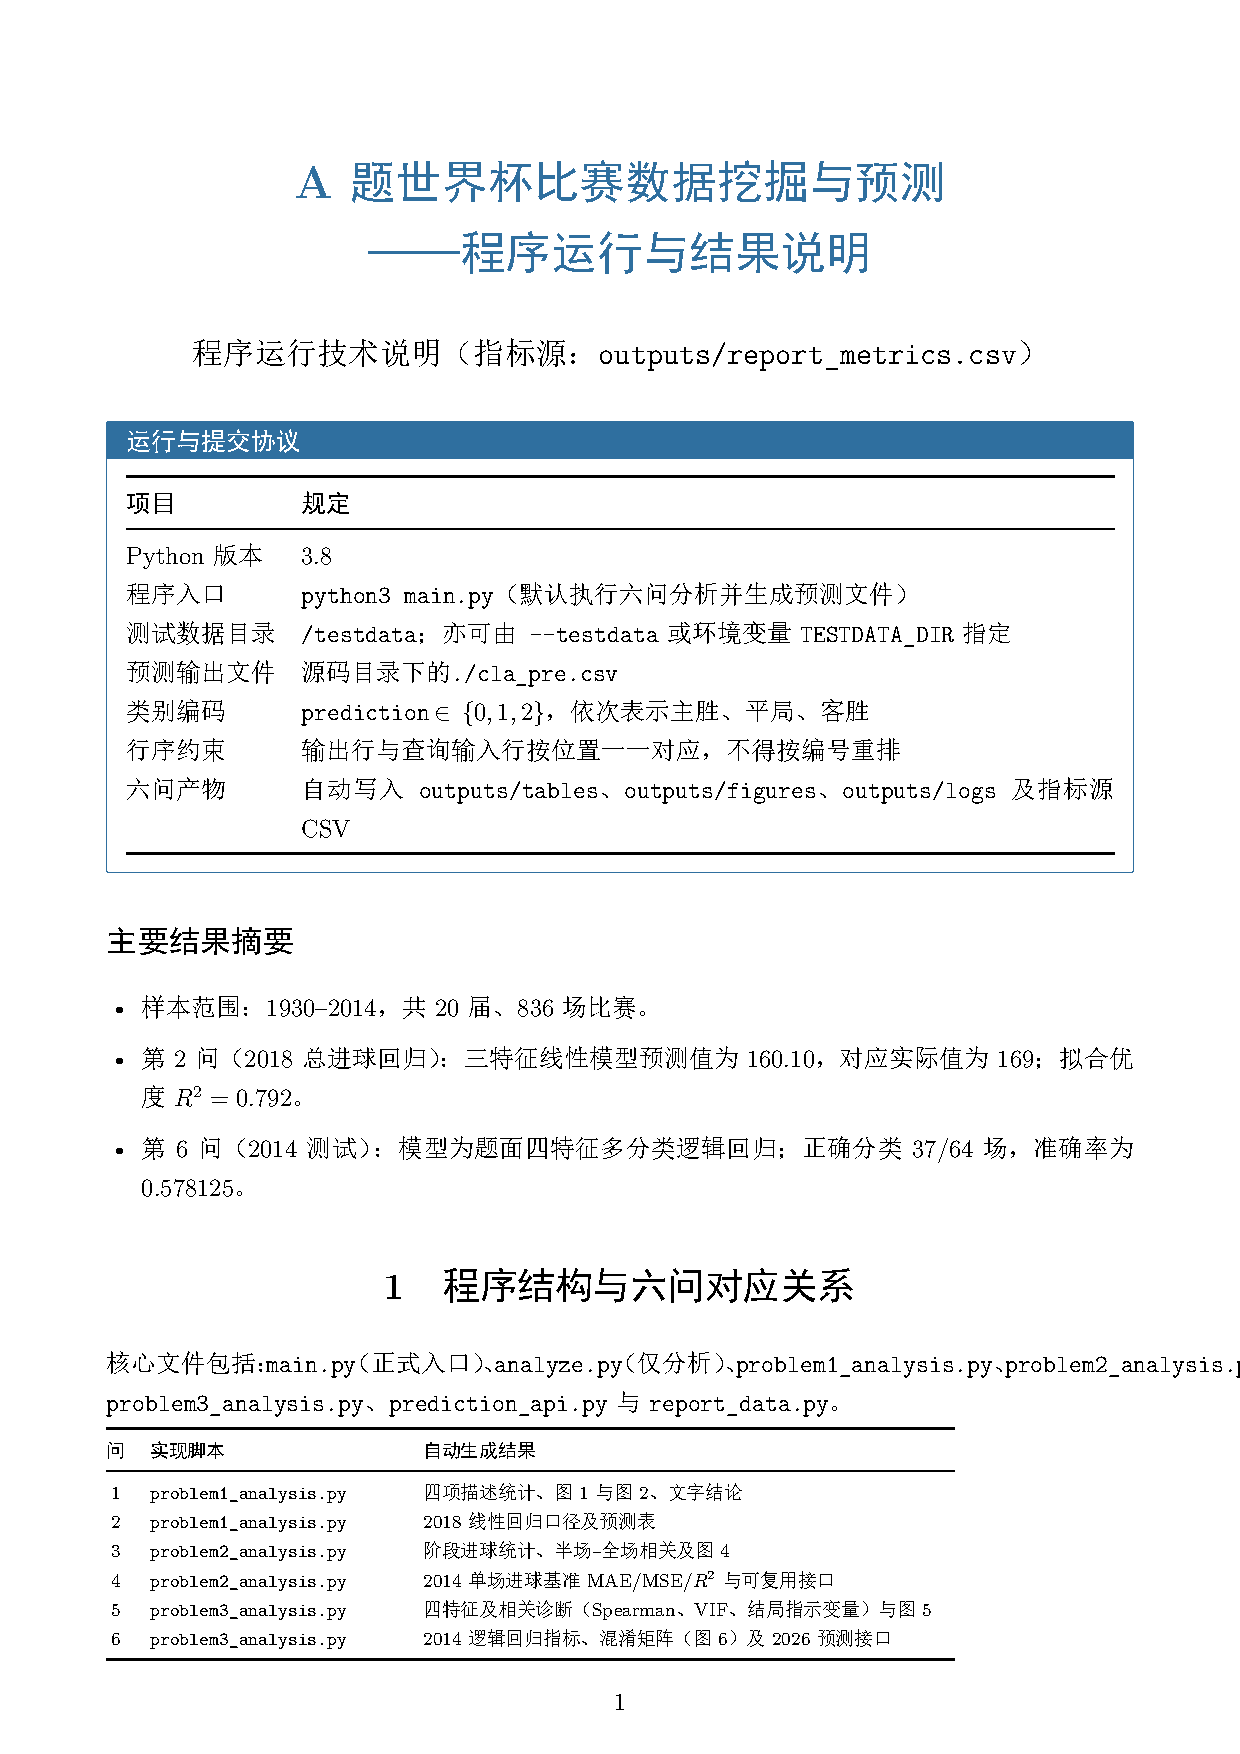
\includepdf[pages=-]{../contest_program_notes_zh.pdf}
\pdfbookmark[0]{Part II\quad Post-competition extensions}{part2}
\setcounter{page}{1}
\exthead{World Cup match data mining and prediction}
\begin{center}{\Large\bfseries Part II\quad Post-competition extensions}\end{center}

The problem asks for descriptive statistics, a regression of total goals, a prediction of goals per match and a win--draw--loss classification based on World Cup data for 1930--2014. The submitted program reaches a classification accuracy of 0.578 on the 64 matches of 2014. Three World Cups have been played since the contest data end: 2018 (64 matches), 2022 (64 matches) and 2026 (104 matches, the first with 48 teams). No model could see these 232 matches when it was built, so they form a strict prospective test.

\section{A genuine future hold-out: a prospective test on three World Cups}

\subsection{Design}
The submitted multi-class model is used unchanged, with the team-history features frozen at 2014. As an external benchmark, E1 builds a model that uses information the contest data do not contain: World Football Elo ratings updated match by match over all international matches (more than 49\,000, from the CC0-licensed dataset martj42/international\_results\cite{martj42}), mapped to win, draw and loss probabilities by an ordered logit fitted only on World Cup matches of 1930--2014. Results count after extra time, as in the training data. The evaluation uses the log loss, the ranked probability score (RPS), the Brier score and accuracy, and comparisons use a paired bootstrap over matches (5\,000 resamples).

\subsection{Results}
\begin{table}[htbp]\centering\small
\caption{Prospective performance on the 232 matches of the 2018--2026 World Cups.}\label{tab:wc-e1}
\begin{tabular}{lcccc}\toprule
Model & Log loss & RPS & Brier & Accuracy\\\midrule
Base rate (frequencies of 1930--2014) & 1.064 & 0.235 & 0.644 & 0.440\\
\textbf{Submitted multi-class model (frozen at 2014)} & 1.008 & 0.210 & 0.605 & 0.578\\
Elo benchmark (ordered logit) & 0.950 & 0.191 & 0.556 & 0.578\\
Equal-weight pool (submitted model + Elo) & \textbf{0.946} & 0.192 & 0.559 & \textbf{0.603}\\\bottomrule
\end{tabular}
\end{table}

\begin{figure}[htbp]\centering
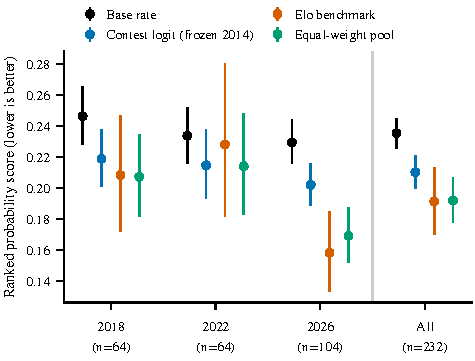
\includegraphics[width=0.6\textwidth]{figE1_prospective_rps.pdf}
\caption{Ranked probability score (RPS) at each World Cup with 95\,\% bootstrap intervals.}\label{fig:wc-e1}
\end{figure}

The submitted model beats the base rate on every proper score, with a log loss lower by 0.056 (95\,\% interval $[-0.094, -0.016]$). Elo beats the submitted model on the RPS ($-0.019$, $[-0.037, -0.0005]$) and the Brier score, while its improvement in log loss ($-0.058$, $[-0.124, +0.009]$) is not significant. The 2022 tournament, full of upsets (Saudi Arabia over Argentina, Japan over Germany and Spain), is the only one at which the history features beat Elo. The equal-weight pool of the two is significantly better than the submitted model alone (log loss $-0.062$, $[-0.092, -0.031]$), which shows that the long-run World Cup record contains information that recent international form does not. Of the 232 matches, 15\,\% involve teams without a World Cup record before 2014 (for example Iceland, Panama, Qatar and Cape Verde), for which the submitted model falls back to a neutral prior.

\section{Where the gap comes from: an improved forecaster frozen before 2018}

\subsection{Question and design}
The submitted classifier was trained with \texttt{class\_weight='balanced'}, a setting that maximises balanced accuracy rather than the quality of the probabilities themselves. On the 232 prospective matches its mean draw probability is 0.332, while the observed draw rate is 0.224. E2 refits forecasters for probability quality, and every candidate is frozen before 2018: regularisation parameters are chosen by leave-one-tournament-out log loss over 1982--2010 (the contest's own selection window), and pooling weights are set by rolling-origin forecasts for 2002--2014.

\subsection{Results}
\begin{table}[htbp]\centering\small\setlength{\tabcolsep}{4pt}
\caption{Performance of the improved forecasters on the 232 matches (ECE: expected calibration error).}\label{tab:wc-e2}
\begin{tabular}{lccccc}\toprule
Model & Log loss & RPS & Brier & Accuracy & ECE\\\midrule
Submitted model (balanced class weights) & 1.008 & 0.210 & 0.605 & 0.578 & 0.126\\
Same four features, refitted without reweighting & 0.944 & 0.191 & 0.555 & 0.586 & 0.035\\
Elo benchmark (ordered logit) & 0.950 & 0.191 & 0.556 & 0.578 & 0.042\\
Equal-weight pool (submitted model + Elo) & 0.946 & 0.192 & 0.559 & \textbf{0.603} & 0.064\\
Learned pool (weight 0.10 on the submitted model) & 0.942 & 0.190 & 0.553 & 0.578 & 0.032\\
\textbf{Combined logit (four features + pre-match Elo difference)} & \textbf{0.936} & \textbf{0.186} & \textbf{0.544} & 0.595 & \textbf{0.030}\\\bottomrule
\end{tabular}
\end{table}

\begin{figure}[htbp]\centering
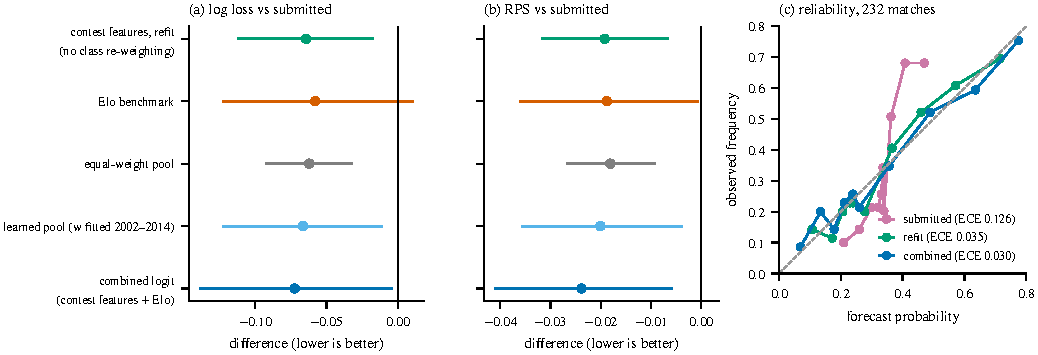
\includegraphics[width=\textwidth]{figE2_improved_forecaster.pdf}
\caption{(a, b) Difference in log loss and RPS of each candidate from the submitted model, with 95\,\% paired bootstrap intervals. (c) Reliability curves of the outcome probabilities (three outcomes pooled, decile bins).}\label{fig:wc-e2}
\end{figure}

Removing the class reweighting alone improves the log loss by 0.064 ($[0.017, 0.112]$) and the RPS by 0.019 ($[0.006, 0.032]$), and it brings the four World Cup history features level with Elo (log-loss difference $-0.006$, $[-0.057, +0.041]$). The gap in E1 therefore comes mainly from the loss function, not from a lack of information. The combined logit is best on all three proper scores and has the lowest calibration error, but its advantage over Elo is not significant on 232 matches: log loss $-0.014$ ($[-0.037, +0.009]$), RPS $-0.005$ ($[-0.011, +0.001]$).

The ranking of the models is not stable across tournaments (Table~\ref{tab:wc-edition}). Split by type of match, the disadvantage of the history features in 2026 comes from matches in which both teams had a World Cup record before 2014 (log loss 0.911 against 0.826, 79 matches); in the 25 matches involving a team without such a record they are in fact better (0.854 against 0.963). A permutation test cannot reject the hypothesis that the gap is the same at every tournament ($p=0.17$). The point estimate of the combined logit is no worse than Elo at any tournament ($-0.005$, $-0.001$, $-0.029$), so it is the more robust single forecaster, not a significantly better one.

\begin{table}[htbp]\centering\small
\caption{Comparison by tournament: log-loss difference from Elo (95\,\% paired bootstrap intervals).}\label{tab:wc-edition}
\begin{tabular}{lcc}\toprule
Tournament & Refitted four features $-$ Elo & Combined logit $-$ Elo\\\midrule
2018 & $-0.007$ $[-0.086, +0.066]$ & $-0.005$ $[-0.043, +0.034]$\\
2022 & $-0.078$ $[-0.162, +0.002]$ & $-0.001$ $[-0.040, +0.044]$\\
2026 & $+0.038$ $[-0.046, +0.121]$ & $-0.029$ $[-0.066, +0.008]$\\\bottomrule
\end{tabular}
\end{table}

\subsection{Conclusions and limits}
The weakness of the submitted model lies not in its features but in its training objective: class reweighting aimed at balanced accuracy systematically inflates draw probabilities, and once probability quality is the objective, the World Cup history supplied by the contest alone reaches the level of the external Elo benchmark. 232 matches are not enough to separate the best few models, so the conclusion should read ``the combined model is more robust'', not ``the combined model is better''. The 2026 tournament used the new 48-team format, and the change of format may itself affect the relative performance of the models.

\begin{thebibliography}{9}
\bibitem{martj42} M. J\"urisoo. International football results from 1872 to present (martj42/international\_results). GitHub, CC0 1.0. \url{https://github.com/martj42/international_results}.
\end{thebibliography}
\end{document}
